%%
% The BIThesis Template for Graduate Thesis
%
% Copyright 2020-2023 Yang Yating, BITNP
%
% This work may be distributed and/or modified under the
% conditions of the LaTeX Project Public License, either version 1.3
% of this license or (at your option) any later version.
% The latest version of this license is in
%   https://www.latex-project.org/lppl.txt
% and version 1.3 or later is part of all distributions of LaTeX
% version 2005/12/01 or later.
%
% This work has the LPPL maintenance status `maintained'.
%
% The Current Maintainer of this work is Feng Kaiyu.
%
% Compile with: xelatex -> biber -> xelatex -> xelatex

\chapter{实验评估 Experimental Evaluation}

本章将对基于强化学习的对抗性恶意样本生成方法进行评估。首先介绍实验的软硬件配置以及用到的评估指标。接下来,展示实验结果,并对模型中每个模块进行对比实验,以验证其可靠性。然后,将该模型与学术界类似任务的模型进行比较。

This chapter evaluates the adversarial malware sample generation method based on RL. First, hardware and software configurations in this experiment and evaluation metrics are introduced. Second, the experimental results are presented, including comparative experiments for each module to verify its reliability. Finally, the proposed model is compared with other models addressing similar tasks in academia.

\section{实验设置 Experiment Setting}

\subsection{实验环境 Experiment Environment}

本文的实验在一台配置为64位Linux操作系统的主机上进行,使用进行计算。本实验在强化学习环境下对恶意软件样本进行策略训练与对抗样本生成,实验平台采用基于 gym-malware 的自定义环境,模拟真实软件行为特征。为了提高训练效率与灵活性,本实验混合使用了 ChainerRL 和 PyTorch 框架。在模型构建方面,使用了 ChainerRL 中的 ACER 和 PPO 算法模块,对 agent 的策略网络与价值网络进行联合优化。环境中使用的样本来由 gym-malware 的接口封装提供动作空间和状态转换功能。为了增强样本多样性,训练过程中使用 EpisodicReplayBuffer 存储历史交互轨迹,并引入时间步奖励衰减机制,具体实验环境如表\ref{tab:5.1}所示。

Experiments in this research were conducted on a host configured with a 64-bit Linux operating system. RL environments were used to train malware samples and generate adversarial samples. The experimental platform utilized a custom environment based on gym-malware to simulate real software behavioral characteristics. To enhance training efficiency and flexibility, the ChainerRL and PyTorch frameworks were jointly employed. For model construction, the ACER and PPO algorithm modules from ChainerRL were used to jointly optimize the agent's policy and value networks. Sample interactions in the environment were managed via gym-malware's interface, which encapsulates action spaces and state transition functionality. To increase sample diversity, the training process uses the EpisodicReplayBuffer to store historical interaction trajectories and introduces a time-step reward decay mechanism. Detailed experimental environment specifications are shown in Table \ref{tab:5.1}.  

\begin{table}[htbp]
	\centering
	\caption{实验环境配置}
	\label{tab:5.1}
	\begin{tabular*}{0.9\textwidth}{@{\extracolsep{\fill}}cc}
		\toprule
		软硬件环境 & 具体配置信息\\
		\midrule
		CPU & Intel i7-12700 \\
		内存 & 32GB \\
		操作系统 & Ubuntu 20.04.3 LTS \\
		\multirow{4}{*}[0.5em]{开发环境} & Python 3.6 \\
		& ChainerRL 0.7.0 \\
		& LIEF 0.12.3 \\
		& Gym 0.9.2 \\
		\bottomrule
	\end{tabular*}
\end{table}

\subsection{数据集构建 Dataset Construction}

在使用指令替换作为扰动方法时,由于不同处理器架构所使用的指令集存在差异,因此在构建数据集时必须确保所有样本来自同一处理器架构。当前 Linux 平台的恶意软件主要针对 ARM、x86-64、MIPS 等常见架构,其中 x86-64 是最广泛使用的目标平台。考虑到本研究的指令替换环境是基于x86架构指令集的,故本文统一选择 x86-64 架构的 Linux ELF 文件作为研究对象。其中,恶意样本来源于 VirusShare 网站,良性样本则提取自本实验所使用的 Ubuntu 系统。

When employing instruction substitution as a disturbance method, all samples should originate from the same architecture because instruction sets used by different processor architectures have differences. Current Linux malware primarily targets common architectures, such as ARM, x86-64, and MIPS, with the condition that x86-64 has been the most widely adopted platform. Given that this research's instruction substitution environment is based on the x86 instruction set, all Linux ELF files selected for analysis are of the x86-64 architecture. Malicious samples were sourced from the VirusShare website, while benign samples were extracted from the Ubuntu system used in this experiment.

本节系统介绍了本研究所使用的数据集构建过程。在当前缺乏公开标准 Linux ELF 恶意/良性软件数据集的背景下,本文采用“自主收集 + 多重筛选”的方式构建了一个规模适中、质量较高的专用数据集。具体而言,首先从 VirusShare 平台中收集了 43,553 个原始恶意 ELF 样本,并经过架构筛选和 objdump 反汇编能力检测,最终保留13,845 个结构完整的 x86架构的恶意样本。

This section details the dataset construction process. In the absence of publicly available standard Linux ELF malware and benign software datasets, this research constructs a moderate-scale, high-quality dedicated dataset by using self-collection and multi-step sifting methods. Specifically, 43,553 raw malicious ELF samples were collected from VirusShare. After sifting by architecture and objdump disassembly capability testing, 13,845 structurally intact x86 malicious samples were retained.

良性样本部分,本研究从实际 Ubuntu 系统环境中提取 /bin、/usr/bin 等路径下的 ELF 可执行文件,经过格式验证和架构确认,获得 2,141个良性 ELF 样本。这些样本代表了正常的系统运行和用户操作,确保了良性与恶意样本在后续训练中的平衡性,并为模型提供了丰富的正常行为数据。

For benign samples, ELF executables from paths such as /bin and /usr/bin were extracted from an actual Ubuntu environment. Format verification and architecture confirmation selected 2,141 benign ELF samples. These represent normal system operations and user activities, ensuring the balance between benign and malicious samples during training and providing abundant behavioral data.

为了保证实验结果的可靠性,本文对所选样本的标签进行了二次验证。具体来说,首先使用Virustotal平台对每个恶意软件样本进行扫描和分析。Virustotal通过多种杀毒引擎和分析工具对上传的文件进行检测,并提供详细的检测报告。基于这些报告,本文可以查看每个样本被各个反病毒引擎标记为恶意软件的情况,以及它们在不同引擎中的检测结果。

To ensure the result reliability, sample labels were conducted the secondary verification. In concrete, first, each malware sample was scanned and analyzed by the VirusTotal platform. VirusTotal scanned the uploaded file using multiple antivirus engines and analysis tools and provided detailed scanning reports. Based on these reports, this research could check the circumstances that each sample was marked as malware by each antivirus engine and the detection results in different engines.

在二次验证过程中,首先检查每个样本在Virustotal平台上的检测结果是否与本文原始收集的标签一致。本文只保留被大于5个反病毒引擎报告为恶意的样本,如果某个样本的检测结果全为良性,本文才保留它作为良性样本,其余的不确定样本都将被剔除。此外,Virustotal还提供了“first-seen”字段,记录了恶意软件样本首次被检测到的时间,结合该字段,本文能够进一步确认样本的来源和是否属于已知的恶意软件家族。

In the secondary verification process, each sample was checked to see whether the detection result from the VirusTotal platform was the same as original labels collected by this research. This research only retained samples that are reported as malware by more than five antivirus engines as malicious samples. If a sample's detection results were all benign, this research retained it as benign samples. Otherwise, VirusTotal offers the “first-seen” field to record when the malicious sample was first detected. Combining this field, this research can further ensure the sample's source and identify whether it belongs to any known malware families.

在构建数据集过程中,除了收集和筛选恶意与良性 ELF 样本外,本文还利用 LIEF 工具从良性样本中提取了扰动的字节,包括字符串数据等。这一过程对于后续对抗样本的生成至关重要。

During the dataset construction process, besides collecting and sifting malicious and benign ELF samples, this research also used LIEF tools to extract bytes for perturbation, such as string data, from benign samples. This process is vital for subsequent adversarial sample generation.

为了确保扰动字节的多样性和有效性,本文从良性样本中提取了不同类型的数据,包括程序的常量字符串、符号信息及其相关的内存布局。通过修改这些字节,生成的对抗样本不仅能够在字节层面改变文件的内容,还能在功能上对检测模型产生干扰。这些经过扰动处理的字节经过 LIEF 工具的再次封装,确保它们仍然符合 ELF 文件的格式要求,避免破坏文件的整体结构,保证生成的对抗样本在有效性和可执行性之间保持平衡。此部分操作为构建一个高效且可靠的对抗训练模型提供了坚实的数据支持。

To ensure the diversity and validity of bytes for perturbation, this research extracted different types of data from benign samples, such as program constant strings, symbol information, and related memory layouts. By modifying these bytes, generated adversarial samples can not only alter the file's content at byte level but also disturb  detection models in functionality realm. These disturbed bytes re-encapsulated by LIEF tools ensured that they still fit ELF file format requirements, avoiding disruption of overall file structures, maintaining the balance between validity and executability. These operations provided solid data support for constructing an effective and reliable adversarial training model.

经过标签验证、时间戳的信息获取,本文最终构建了实验所用的数据集,如表\ref{tab:5.2}所示,该数据集将用于后续章节中的特征建模、状态空间构造、动作空间设计与策略训练等关键任务,并为本研究探索基于强化学习的恶意样本对抗生成技术奠定了坚实的基础。

Through label verification and timestamp validation, this research constructed the experimental dataset, which is listed in Table \ref{tab:5.2}. It will facilitate crucial tasks such as feature modeling, state space construction, action space design, and policy training, constructing a solid foundation for exploring adversarial malware generation methods based on RL.  

\begin{table}[htbp]
	\centering
	\caption{数据集信息统计}
	\label{tab:5.2}
	\begin{tabular*}{0.9\textwidth}{@{\extracolsep{\fill}}ccc}
		\toprule
		数据集类型 & 样本数量 & 时间跨度 \\
		\midrule
		恶意样本 & 8456 & 2014.06--2020.04 \\
		良性样本 & 2054 & 2016.12--2018.08 \\
		\bottomrule
	\end{tabular*}
\end{table}

\subsection{特征处理方式 Feature Processing Approach}

在恶意软件检测任务中,特征提取是一项关键的前置工作,它能够在不执行程序的前提下,从可执行文件的结构和内容中挖掘具有判别力的信息。本项目面向ELF(Executable and Linkable Format)格式的Linux恶意样本,因为数据集的特殊性,本文基于LIEF(Library to Instrument Executable Formats)库构建了一个可扩展的静态特征提取模块,融合了多种维度的特征,用于后续的机器学习与强化学习模型训练。

In malware detection tasks, feature extraction is a critical preprocessing step that enables extracting discriminative information from executable files' structures and contents without executing the program. Targeting Linux malicious samples in ELF, this project constructed an extensible static feature extraction module based on the LIEF library due to the dataset’s specificity. This module integrates multi-dimensional features for subsequent machine learning and RL model training.

该模块采用面向对象的结构设计,核心思想是为每种特征类型设计一个独立的类,实现特征提取的解耦与模块化。每个特征类负责从原始ELF样本中提取特定的信息,输出为结构化的特征向量或统计指标。最终,所有特征被组合为一个统一的特征向量,供模型使用。该方法具有通用性强、计算效率高、不依赖动态执行环境等优点,适用于大规模样本处理与对抗样本生成任务,具体特征类型如表\ref{tab:5.3}所示。

This module adopts an object-oriented structure design. Its core idea is designing an independent class for each feature type to achieve decoupling and modularization for feature extraction. Each feature class is responsible for extracting specific information from original ELF samples and outputting structured feature vectors or statistical metrics. Ultimately, all features combine into a unified feature vector for model usage. This method exhibits advantages, including high generalizability, computational efficiency, and independence from dynamic execution environments, making it suitable for large-scale sample processing and adversarial sample generation tasks. Specific feature types are listed in Table \ref{tab:5.3}.  

\begin{table}[htbp]
	\centering
	\caption{静态特征类别及其描述}
	\label{tab:5.3}
	\begin{tabular*}{\textwidth}{@{\extracolsep{\fill}}cc>{\centering\arraybackslash}m{7cm}}
		\toprule
		特征类别 & 特征名称/维度 & 特征描述 \\
		\midrule
		字节频率直方图 & ByteHistogram(256维) & 统计文件中每种字节值(0$\sim$255)出现的次数,并进行归一化。此特征能反映文件在字节层面的分布特性,如是否压缩、加密等。 \\
		
		熵-字节二维直方图 & ByteEntropyHistogram(2D) & 将文件分成固定大小窗口,分别计算每个窗口的熵值和各字节的分布,生成二维直方图。用于反映局部内容复杂度和结构变化。 \\
		
		节区统计特征 & SectionInfo(变长) & 提取节区名称、大小、熵值、可执行标志等,统计各节区出现次数、大小分布及权限类型,可分析文件布局规律与异常结构。 \\
		
		导入函数特征 & Imports(变长) & 提取程序使用的所有外部导入函数(如 libc 函数),构建 API 调用集合,可反映样本行为意图。 \\
		
		ELF头部信息特征 & Header(固定维度) & 提取如文件类型(ET\_EXEC/ET\_DYN)、架构类型(如 x86、ARM)、入口地址、节区偏移、程序头数量等元数据。 \\
		\bottomrule
	\end{tabular*}
\end{table}



\subsection{检测器训练与评估  Detector Training and Evaluation}

本章基于表\ref{tab:5.2} 所示的训练集和表\ref{tab:5.3} 所示的特征提取方式,训练基于随机森林(Random Forest, RF)和SVM的 Linux ELF 恶意软件检测器,并利用测试集对这些检测器进行了评估。为了全面衡量模型性能,本研究采用四种常见的机器学习评价指标:精确率(Precision)、准确率(Accuracy)、召回率(Recall)以及 F1 分数(F1-score)。这些评价指标的计算公式如公式(5.1)至(5.4)所示:

Using the training set illustrated in Table 5-2 and the feature extraction methods presented in Table 5-3, this chapter trains Linux ELF malware detectors based on Random Forest (RF) and SVM and evaluates these detectors using the test set. To comprehensively assess model performance, this research adopts four common machine learning evaluation metrics, including precision, accuracy, recall, and F1-score. The calculation formulations for these metrics are shown in equations (5.1) to (5.4):
\begin{equation}
	\text{Precision} = \frac{TP}{TP + FP}
	\tag{5.1}
\end{equation}
\begin{equation}
	\text{Accuracy} = \frac{TP + TN}{TP + FP + TN + FN}
	\tag{5.2}
\end{equation}
\begin{equation}
	\text{Recall} = \frac{TP}{TP + FN}
	\tag{5.3}
\end{equation}
\begin{equation}
	F_1 = 2 \times \frac{\text{Precision} \times \text{Recall}}{\text{Precision} + \text{Recall}}
	\tag{5.4}
\end{equation}

其中,TP 表示真实为恶意且被正确识别为恶意的样本数量;FP 表示真实为良性
却被错误分类为恶意的样本数量;TN 表示真实为良性且被正确分类为良性的样本数
量;FN 表示真实为恶意却被误分类为良性的样本数量。

In the formulations, TP denotes the number of samples correctly identified as malicious. FP represents the number of benign samples incorrectly classified as malicious. TN denotes the number of benign samples correctly classified as benign. FN represents the number of malicious samples incorrectly classified as benign.

基于上述指标,本文对随机森林和 SVM 检测器在测试集上的性能进行了评估,
评估结果如表\ref{tab:5.4}所示。实验结果表明,基于随机森林的检测器和 SVM 均取得了较
高的检测性能,四项评价指标普遍超过 96\%。随机森林(RF)在四项性能指标中均
优于支持向量机(SVM),尤其在准确率和召回率方面具有明显优势。其中,RF 检
测器的准确率达到 99.0\%,精确率与召回率分别为 99.0\% 和 97.0\%,F1 分数也高达
98.0\%,表明其在保持低误报率的同时,具备较强的漏报控制能力。相比之下,SVM 虽
然也表现出良好的检测能力,其准确率和精确率略低,为 97.0\% 和 96.0\%,召回率
和 F1 分数为 96.5\% 和 97.5\%,在部分样本的分类上略逊一筹。这说明随机森林模
型在处理复杂的高维特征数据时具有更强的鲁棒性和泛化能力,能够更有效地识别恶
意样本。因此,在本研究的数据集和特征设置下,随机森林更适合作为主要的检测模
型。

Based on these metrics, this research evaluates the performance of RF and SVM detectors on the test set. The results are presented in Table \ref{tab:5.4}. The results indicate that both RF and SVM achieved high detection performance, with all four metrics exceeding 96\%. RF precedes SVM across all metrics, particularly in accuracy and recall. RF achieved 99.0\% accuracy, 99.0\% precision, 97.0\% recall, and 98.0\% F1-score. This indicates strong false-negative control while maintaining a low false-positive rate. In comparison, SVM showed robust but slightly inferior result: 97.0\% accuracy, 96.0\% precision, 96.5\% recall, and 97.5\% F1-score, which demonstrates that SVM is inferior to RF in some sample classifications. These results indicate that the RF model exhibits stronger robustness and generalization capabilities when processing complex high-dimensional feature data, enabling more effective malware identification. Therefore, with the dataset and feature configuration of this research, Random Forest is more suitable as the primary detection model.

\begin{table}[htbp]
	\centering
	\caption{目标检测器性能评估}
	\label{tab:5.4}
	\renewcommand{\arraystretch}{1.3}
	\begin{tabular*}{0.9\textwidth}{@{\extracolsep{\fill}}ccccc}
		\toprule
		检测器 & Accuracy & Precision & Recall & F1-score \\
		\midrule
		RF  & 99.0\% & 99.0\% & 97.0\% & 98.0\% \\
		SVM & 97.0\% & 96.0\% & 96.5\% & 97.5\% \\
		\bottomrule
	\end{tabular*}
\end{table}

\subsection{实验评估指标 Experimental Evaluation Metrics}

为了全面评估基于强化学习的对抗样本生成方法的有效性与实用性,本文选取了以下五个核心指标进行分析:攻击成功率、扰动幅度、收敛速度、迁移攻击成功率与平均生成时间。这些指标能够从攻击效果、扰动隐蔽性、训练效率、策略泛化能力以及资源消耗等多个维度对方法进行定量评估。

To comprehensively evaluate the effectiveness and practicality of the adversarial sample generation method based on RL, this study employs the following five core metrics: attack success rate, perturbation count, convergence speed, transfer attack success rate, and average generation time. These metrics enable quantitative assessment across multiple dimensions, including attack efficacy, perturbation concealment, training efficiency, policy generalization capability, and resource consumption.

\begin{enumerate}[label=\arabic*)]
	\item 攻击成功率(Attack Success Rate, ASR) \\
	攻击成功率用于衡量生成的对抗样本是否能够成功欺骗目标检测模型,是最核心的评估指标之一。其定义如下:

    ASR measures whether the adversarial samples successfully deceive the target detection model and is one of the most critical evaluation metrics. Its definition is:
	\begin{equation}
		\text{ASR} = \frac{N_{\text{success}}}{N_{\text{total}}}
		\tag{5.5}
	\end{equation}
	其中,$N_{\text{success}}$ 表示攻击成功的样本数量,$N_{\text{total}}$ 表示总共生成的对抗样本数量。ASR 越高,说明强化学习智能体生成的策略越有效,攻击能力越强。

    In this formulation, $N_{\text{success}}$ denotes the count of samples achieving successful attacks, and $N_{\text{total}}$ presents the total number of adversarial samples generated. A higher ASR indicates greater effectiveness and stronger attack capability of the strategies generated by RL agent.
	
	\item 扰动次数(Perturbation Count) \\
	扰动次数用于衡量生成对抗样本过程中所进行的特征修改的次数。扰动次数越多,代表对抗样本与原始样本的差异越大。该指标有助于评估对抗样本的“隐蔽性”与“攻击强度”。定义为每个对抗样本在生成过程中所使用的扰动动作数量,扰动次数越少,表示对抗样本越隐蔽,攻击的有效性越强。

    Perturbation count measures the number of feature modifications applied during adversarial sample generation. Higher perturbation counts imply greater deviations between adversarial and original samples. This metric helps evaluate the concealment and attack intensity of adversarial samples. It is defined as the number of perturbation actions used per adversarial sample during the adversarial sample generation process. Fewer perturbations indicate higher concealment and stronger attack validity.
	
	\item 收敛速度(Convergence Speed)\\
	收敛速度用于衡量智能体在训练过程中达到预期性能水平(如攻击成功率超过某一阈值)所需的训练步数或时间。其定义如下:

    Convergence Speed measures the training steps or time required for the agent to reach a predefined performance level, such as ASR exceeds a threshold during training. Its definition is:
	\begin{equation}
		S_{\text{converge}} = \min\{t \mid \text{ASR}_t \geq \tau\}
		\tag{5.6}
	\end{equation}
	其中,$\text{ASR}_t$ 表示第 $t$ 步时的攻击成功率,$\tau$ 为设定的阈值(如 90\%)。收敛速度越快,说明训练过程越高效,可节省计算资源和实验时间。

    In this formulation, $\text{ASR}_t$ denotes the attack success rate at step $t$, and $\tau$ represents the preset threshold such as 90\%. Faster convergence indicates higher training efficiency and reduces computational resource consumption and training time.
	
	\item 迁移攻击成功率(Transfer Attack Success Rate, TASR)\\
	迁移攻击成功率用于衡量训练完成的对抗策略是否具有较好的泛化能力,即能否成功攻击其他未见过的目标模型。定义如下:

    TASR measures the generalization capability of the trained adversarial strategy that whether it can successfully attack other unseen target models or platforms. Its definition is:
	\begin{equation}
		\text{TASR} = \frac{N_{\text{transfer\_success}}}{N_{\text{transfer\_total}}}
		\tag{5.7}
	\end{equation}
	其中,$N_{\text{transfer\_success}}$ 表示在新模型或平台上攻击成功的样本数量,$N_{\text{transfer\_total}}$ 为参与迁移测试的样本总数。TASR 越高,表明策略具备更好的泛化能力。

    In this formulation, $N_{\text{transfer\_success}}$ denotes the count of samples successfully attacking new models or platforms, and $N_{\text{transfer\_total}}$ represents the total number of samples tested for transferability. Higher TASR indicates stronger generalization capability.
	
	\item 平均生成时间(Average Generation Time)\\
	平均生成时间反映了每个对抗样本从生成到验证所需的时间,代表方法的实际可用性。其定义如下:

    Average Generation Time reflects the time required to generate and verify each adversarial sample, representing the method's practical usability. Its definition is:
	\begin{equation}
		T_{\text{avg}} = \frac{1}{N} \sum_{i=1}^{N} T_i
		\tag{5.8}
	\end{equation}
	其中,$T_i$ 表示第 $i$ 个样本的生成时间,$N$ 为总样本数量。生成时间越短,说明该方法更适合实际部署或大规模生成场景。

    In this formulation, $T_i$ denotes the generation time for Sample $i$, and $N$ represents the total sample count. Shorter generation times indicate greater suitability for practical deployment or large-scale generation scenarios.
\end{enumerate}

\section{恶意软件对抗性生成模型表现 Performance of Adversarial Malware Generation Model}

在本实验中,训练和测试样本的选择过程是基于Virustotal报告中的“first-seen”字段进行排序的。该字段记录了每个恶意软件样本第一次被Virustotal平台发现的时间,代表了该样本首次出现的日期和时间。通过利用这一时间戳,能够对样本进行时间上的排序,从而模拟恶意软件的进化过程。

In this experiment, the selection process of training and testing samples was sorted based on the "first-seen" field from VirusTotal reports. This field records the date and time when each malware sample was first scanned by the VirusTotal platform, representing its initial appearance. Utilizing these timestamps allows that malware revolution can be simulated by sorting samples in time ordering.

具体来说,本文首先从Virustotal平台获取了大量恶意软件样本的检测报告,并依据“first-seen”字段对这些样本进行了升序排序。检测模型和对抗样本生成模型使用不同的数据,检测模型使用位于时间序列前端的数据训练,对抗样本生成模型则使用位于后端的数据。这一排序策略的优势在于,它能够帮助本文训练模型识别早期和新兴的恶意软件样本,进而提升模型在面对新型、未被广泛识别的恶意软件时的适应能力。通过选择“first-seen”较早的样本作为训练集,能够确保模型能够处理那些相对较早出现的恶意软件,并从这些样本中学习到潜在的攻击模式。

Specifically, this research gathered numerous malware sample detection reports and sorted them in ascending order according to the "first-seen" field. The detection model and adversarial sample generation model utilize different datasets. The detection model used data situated at the front of time sequence for training while the adversarial sample generation model used data located at the end of time sequence. This sorting strategy exhibits advantages in promoting the training model in this research to identify historical and newly emerging malware samples, thus enhancing the model's adaptivity for novel malware that are not detected widely. Selecting earlier "first-seen" samples ensures that models can address malware that earlier presented, learning potential attack approaches from these samples.

在测试集的选择上,本文同样使用了“first-seen”字段对样本进行排序,确保测试集包含来自不同时间段的恶意软件样本。这种方法使得模型不仅能够评估其在新样本上的表现,还能够检测其在历史样本上的有效性。通过这种方式,研究者能够全面地考察模型在多种恶意软件类型和攻击模式下的泛化能力。

For test set selections, this research also utilizes the "first-seen" field to sort samples to ensure that test dataset includes malware from diverse time periods. This method stimulates models not only to evaluate their performance on different novel samples but also to examine the validity of historical samples. Researchers can comprehensively examine generalization capabilities across multiple malware types and attack patterns.

\subsection{参数选择 Parameter Selection}

在本实验中,本文对强化学习模型的参数进行了精心设置,以确保训练过程的有效性和稳定性。以下是关键参数的设置和说明:
首先,训练的步骤数(rounds)设定为5000至10000步,目的是确保智能体通过足够的交互时间学到有效的策略。每个步骤代表智能体与环境的一次交互,智能体根据当前的策略选择动作并根据奖励更新其策略。训练的过程中,本文使用了两种不同的环境:malware-v0和malware-score-v0。malware-v0是一个没有评分机制的环境,而malware-score-v0则包含了评分系统,用于模拟黑盒攻击和白盒攻击两个环境,常见具体的参数如表\ref{tab:5.5}所示。

In this experiment, the parameters of RL model were meticulously configured to ensure effective and stable training. Critical parameter settings and descriptions are introduced as follows: The number of training rounds was set between 5,000 and 10,000 to ensure sufficient interaction time for the agent to learn effective strategies. Each step represents an interaction between the agent and the environment. The agent selects an action based on its current policy and updates the policy according to the reward. During training, two distinct environments were used: malware-v0 and malware-score-v0. malware-v0 is an environment lacking a scoring mechanism, while malware-score-v0 incorporates a scoring system to simulate black-box and white-box attack environments. Common specific parameters are listed in Table \ref{tab:5.5}.

\begin{table}[htbp]
	\centering
	\caption{模型超参数}
	\label{tab:5.5}
    \begin{tabular*}{0.9\textwidth}{@{\extracolsep{\fill}}ccc}
    \toprule
		超参数 & 数值 & 说明 \\
    \midrule
		学习率 & 0.0003 & 控制每次参数更新的步长,值越小,更新越稳定 \\
		折扣因子 & 0.99 & 奖励的时间折扣因子,值越大代表对未来奖励越看重 \\
		GAE 参数 & 0.95 & 广义优势估计(GAE)中的参数,用于平衡偏差与方差 \\
		批大小 & 2048 & 每次从环境中收集的样本数量,用于一次策略更新 \\
		Epoch 数 & 10 & 每次策略更新所进行的训练轮数,用于提升收敛效果 \\
		剪切范围 & 0.2 & 用于限制策略更新幅度的剪切参数,防止策略剧烈更新\\
		优化算法 & Adam & 用于梯度下降的优化器,具有自适应学习率的能力 \\
    \bottomrule
	\end{tabular*}
\end{table}

在模型架构方面,PPO模型使用了带LSTM(长短期记忆)层的架构,以便于处理带有时间相关性的任务。模型的输入是来自环境的状态信息,经过全连接层后输入到LSTM层,LSTM层帮助智能体记住长期的信息,并且输出动作的概率分布(pi)和状态价值估计(v)。该模型的隐藏层大小为128,LSTM层的输出维度与隐藏层大小相同。

In the model architecture aspect, the PPO model employed a structure with LSTM layers to handle temporally correlated tasks. The model input consists of state information from the environment, processed through a fully connected layer before entering the LSTM layer. The LSTM layer enables the agent to retain long-term information and outputs a probability distribution pi of actions and the state value estimate v. The hidden layer size of this model is 128, which is equivalent to the output dimension of the LSTM layer.

确认好超参数,将LSTM层数分别设置为1、2、3、4,训练10个epoch,记录每组模型在同一检测器下的平均逃逸率、标准差(衡量模型稳定性)和平均训练步数。实验使用1500个恶意样本作为训练集,训练目标是通过最小化被检测器发现的概率生成对抗样本,实验结果如表\ref{tab:5.6}所示。

After confirming the hyperparameters, the number of LSTM layers was set to 1, 2, 3, and 4, respectively. Each configuration was trained for 10 epochs, with the average evasion rate, standard deviation that indicates model stability, and average training steps recorded by the same detector. The experiment utilized 1500 malicious samples as the training set, with the target of generating adversarial samples by minimizing their detection probability. Experimental results are presented in Table \ref{tab:5.6}.  

从实验结果可见,随着LSTM层数的增加,模型的表达能力逐渐增强,在一定程度上有助于提升逃逸率。从表\ref{tab:5.6}可以看出,随着 LSTM 层数从1层增加到3层,平均逃逸率从85.4\%上升到89.1\%,平均扰动数也从 3.1 次增至 4.2 次,说明更深的时序模型能够捕捉更丰富的策略特征,提高对抗样本的生成效果。与此同时,收敛速度在 2 层时达到最快(4500步),而在 3 层和 4 层时分别回升至4600步和5200步,表现出过深网络带来的训练效率下降。

From the experimental results, it is evident that as the number of LSTM layers increases, the model's representational capacity gradually strengthens, which contributes to improving the evasion rate to a certain extent. As shown in Table \ref{tab:5.6}, when the number of LSTM layers increases from 1 to 3, the average evasion rate rises from 85.4\% to 89.1\%, and the average number of perturbations increases from 3.1 to 4.2, demonstrating that deeper temporal models capture more abundant strategic features, enhancing adversarial sample generation efficiency. Meanwhile, convergence speed is fastest at 2 layers (4500 steps) but increases to 4600 and 5200 steps at 3 and 4 layers, respectively, indicating reduced training efficiency due to excessive network depth.

\begin{table}[htbp]
	\centering
	\caption{参数选择:不同LSTM层数的实验结果}
	\label{tab:5.6}
	\begin{tabular*}{0.9\textwidth}{@{\extracolsep{\fill}}cccc}
		\toprule
		LSTM 层数 & 平均逃逸率(\%) & 平均扰动数(次) & 收敛速度(步) \\
		\midrule
		1 & 85.4 & 3.1 & 5000 \\
		2 & 88.7 & 3.8 & 4500 \\
		3 & 89.1 & 4.2 & 4600 \\
		4 & 87.5 & 4.5 & 5200 \\
		\bottomrule
	\end{tabular*}
\end{table}

综合来看,2层LSTM不仅实现了较高的逃逸率(88.7\%)和适中的扰动成本(3.8 次),还在收敛速度上表现最优,因此在攻击效果和训练效率之间取得了最佳平衡。基于此,本文最终采用2层LSTM作为策略网络的核心结构,用于高效生成对抗样本。

Overall, the 2-layer LSTM achieves a high evasion rate (88.7\%) and moderate perturbation cost (3.8 times) while exhibiting optimal convergence speed. This configuration strikes the best balance between attack effectiveness and training efficiency. Based on this result, this study adopts the 2-layer LSTM as the core architecture of the policy network for efficient adversarial sample generation.

确认好 LSTM 层数后,隐藏层的大小对模型的对抗样本生成性能也有显著影响。实验分别设置了隐藏层大小为 64、128、256、512,并在相同条件下对比了攻击成功率、平均扰动数和收敛速度等指标,结果如表\ref{tab:5.7} 所示。随着隐藏层规模从 64 增大到 256,攻击成功率从 85.4\% 提升至 89.1\%,平均扰动数也由 2.9 次增加到 4.1 次,说明更大的隐藏层能够捕捉更丰富的特征信息,从而提高对抗样本的生成效果。但当隐藏层大小进一步增至512时,攻击成功率出现回落(87.5\%),且收敛速度由最佳的4500步增至5200步,表明过大的网络容量容易导致训练效率下降。

After confirming the LSTM layer count, the hidden layer size significantly affects adversarial sample generation performance. Experiments compared hidden layer sizes of 64, 128, 256, and 512 under the same conditions, evaluating attack success rate, average perturbation frequency, and convergence speed. The results are shown in Table 5-7. As the hidden layer size increased from 64 to 256, attack success rate improved from 85.4\% to 89.1\%, and average perturbation times rose from 2.9 to 4.1, indicating that larger hidden layers capture more abundant feature information to enhance adversarial sample quality. However, when the size increased to 512, attack success rate dropped to 87.5\%, and convergence slowed from the optimal 4500 steps to 5200 steps, confirming that excessive network capacity reduces training efficiency.

综合来看,隐藏层大小为 128 时,模型在攻击成功率(88.7\%)、平均扰动数(3.8次)以及 收敛速度(4500步)三个指标上均取得了最佳平衡,既保证了较高的逃逸效果,又保持了较快的训练收敛。因此,结合前述 LSTM 层数的选择,本文最终采用由两层 LSTM 组成、每层隐藏单元数为 128 的网络结构,作为对抗样本生成策略的核心模型。

In summary, when the hidden layer size is 128, the model achieves optimal balance among the success rate of 88.7\% , average perturbations of 3.8 times, and convergence speed of 4,500 steps, not only maintaining high evasion effectiveness but also converging rapidly during training. Therefore, combining the LSTM layer selection discussed before, this research ultimately adopts a network structure constituted by 2 LSTM layers that each contains 
128 hidden units as core adversarial sample generation model.

训练过程中的另一个重要超参数是“标准化优势函数”,这项设置有助于减少由于优势函数估计不准带来的训练不稳定。熵正则化系数(entropy\_coef=0.01)也被设置为0.01,以鼓励策略的多样性,避免智能体过早地陷入局部最优解。

Another critical hyperparameter during training is the standardized advantage function, which helps reduce training instability caused by inaccurate advantage function estimation. The entropy regularization coefficient (entropy\_coef) was set to 0.01 to encourage policy diversity and prevent premature convergence to local optima.

\begin{table}[htbp]
	\centering
	\caption{参数选择:不同隐藏层大小的实验结果}
	\label{tab:5.7}
	\begin{tabular*}{0.9\textwidth}{@{\extracolsep{\fill}}cccc}
		\toprule
		隐藏层大小 & 平均逃逸率(\%) & 平均扰动数(次) & 收敛速度(步数) \\
		\midrule
		64  & 85.4 & 2.9 & 5300 \\
		128 & 88.7 & 3.8 & 4500 \\
		256 & 89.1 & 4.1 & 4700 \\
		512 & 87.5 & 4.6 & 5200 \\
		\bottomrule
	\end{tabular*}
\end{table}

为了选取为了适应训练过程中的策略演化与环境变化,本方法引入奖励权重的自适应调整机制,为了确定动态奖励函数的权重选择,本文设计不同的权重值对比实验,从样本中选取100个样本进行逃逸训练的随机森林模型,实验结果如表\ref{tab:5.8}所示。

To adapt to strategy evolution and environmental changes during the training process, this research introduces an adaptive adjustment mechanism for reward weights. To determine weight selections for the dynamic reward function, this research designs comparison experiments with different weight values. A random forest model was trained using 100 samples for evasion testing, with results presented in Table \ref{tab:5.8}.

\renewcommand{\arraystretch}{1.3}
\begin{table}[htbp]
	\centering
	\caption{参数选择:动态奖励函数不同权重实验结果}
	\label{tab:5.8}
	\begin{tabular*}{0.9\textwidth}{@{\extracolsep{\fill}}cccc}
		\toprule
		序号 & 奖励权重组合($\lambda_1$, $\lambda_2$, $\lambda_3$) & 规避率 & 扰动成本 \\
		\midrule
		1 & (0.9, 0.05, 0.05) & 93.1\% & 6.8 \\
		2 & (0.75, 0.2, 0.05) & 92.4\% & 5.2 \\
		3 & (0.7, 0.25, 0.1) & 89.2\% & 3.1 \\
		4 & (0.6, 0.3, 0.1) & 88.1\% & 2.6 \\
		5 & (0.4, 0.4, 0.2) & 85.7\% & 2.8 \\
		6 & (0.3, 0.2, 0.5) & 80.3\% & 2.4 \\
		\bottomrule
	\end{tabular*}
\end{table}

根据实验数据,设定参数分为三个时期,训练阶段如下:

Based on experimental data, parameters are divided into three phases and listed as follow:

探索期(Exploration Phase):前期以提升规避能力为目标,权重配置为:$\lambda_1= 0.75, \lambda_2 = 0.2, \lambda_3=0.05$

Exploration Phase: Initial stage focused on improving evasion capability:$\lambda_1= 0.75, \lambda_2 = 0.2, \lambda_3=0.05$

收敛期(Exploitation Phase):中期鼓励智能体学习生成稳定有效的低代价策略:

Exploitation Phase: encouraging agent generating stable efficient low-cost strategies in the middle stage :
$\lambda_1= 0.6, \lambda_2 = 0.3, \lambda_3=0.1$

混淆优化期(Confusion Enhancement Phase):后期强化行为混淆性,提高对抗能力隐蔽性:
Confusion Enhancement Phase:  strengthening behavioral confusion to improve concealment in the final stage:
$\lambda_1= 0.4, \lambda_2 = 0.4, \lambda_3=0.2$

\subsection{总体表现 Overall Performance}

确认好模型训练相关的参数之后,本文使用自己所创建的数据集从中选取1000个样本进行实验,训练过程如图所示。为了体现对比度,在本实验中,本文对比了两种强化学习算法,分别是PPO(Proximal Policy Optimization)和ACER\cite{wang2016sample}(Actor-Critic with Experience Replay),以评估它们在恶意软件对抗生成中的表现。PPO作为一种基于策略梯度的方法,强调通过调整策略的更新幅度来保证训练的稳定性。而ACER则结合了策略优化和经验回放的优势,通过信任域优化(Trust Region Optimization)来提高策略的稳定性,同时在训练过程中使用了重放缓冲区来加强对经验的学习。

After setting model training parameters, this research conducts experiments using 1,000 samples from the self-constructed dataset. The training process is shown in the figure. To embody the contrast, this research compares the PPO(Proximal Policy Optimization) algorithm and the ACER(Actor-Critic with Experience Replay)\cite{wang2016sample} algorithm to assess their performance in the adversarial sample generation process. As a method based on policy gradient, PPO emphasizes keeping training stable through adjusting strategy update magnitudes while ACER combines advantages in policy optimization and experience replay, improving strategy's stability through trust region optimization. Meanwhile, buffer replay is also adopted to enhance experiential learning.

从表\ref{tab:5.9}可以看出,所提出的多维度策略优化模型(MPLO)在对抗样本生成任务中表现出显著优势。首先,MPLO 的攻击成功率达到了88.7\%,相比于传统的PPO 方法提升了6.4个百分点,也比 ACER 高出了4.2个百分点,说明 MPLO不仅能够更精准地识别出检测器的决策边界,还能针对性地生成更加隐蔽且有效的扰动。

As shown in Table \ref{tab:5.9}, the proposed Multidimensional Policy Optimization (MPLO) model exhibits significant advantages in adversarial sample generation tasks. MPLO's attack success rate reaches 88.7\%, surging 6.4\% higher than traditional PPO methods and 4.2\% than ACER. This result presents that MPLO can not only recognize the decision-making boundaries of detectors more precisely but also target generating perturbations that are more concealed and effective.
\begin{figure}[hbt]
	\centering
	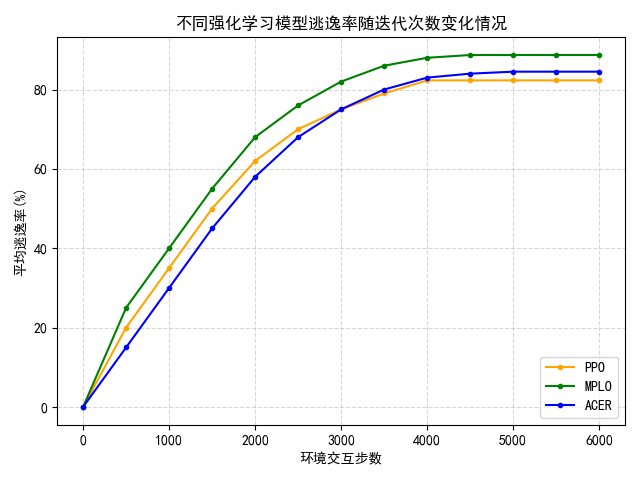
\includegraphics[width=0.75\textwidth]{figures/5.1}
	% \caption[这里的文字将会显示在 listoffigure 中]{这里的文字将会显示在正文中}
	\caption{不同强化学习模型性能训练对比图}\label{fig:5.1}
\end{figure}

其次,MPLO 在修改代价方面同样具有竞争力。它的平均扰动数为3.8次,仅略高于PPO的3.2次,显著低于ACER的4.1次。这表明,在生成同等数量的对抗样本时,MPLO 能以更少的操作步骤完成目标,减少了对原始文件结构的破坏,提高了生成对抗样本的隐蔽性和功能保留度。

In the modification cost aspect, MPLO are also comparative. Its average perturbation time is 3.8, slightly higher than 3.2 of PPO, extremely lower than 4.1 of ACER, indicating that MPLO can complete the goal with lower operation steps at the premise that different models generate same amount adversarial samples, reducing original file structure disruption, improving the generated samples' concealment and functional retention.

最后,从收敛速度来看,MPLO在4500步时就已实现策略稳定,虽然略慢于PPO(4200步),但明显快于ACER(5000步)。这一表现反映了MPLO 在策略更新和经验利用上的高效平衡:通过多维度策略评估机制,它能在探索和利用之间保持良好节奏,快速逼近最优扰动策略,而无需进行过度的样本回放或过长的训练迭代。

Considering the convergence speed, MPLO achieves policy convergence at 4,500 steps, slower than 4,200 steps of PPO but faster than 5,000 steps of ACER, reflecting that MPLO gets an effective balance between exploration and exploitation. Through multi-dimensional strategy evaluation mechanisms, it can maintain the balance between exploration and exploitation, rapidly approaching optimal disturbance strategies without requiring excess sample replay and exceeding training iterations.

\begin{table}[htbp]
	\centering
	\caption{强化学习模型性能对比}
	\label{tab:5.9}
	\begin{tabular*}{0.9\textwidth}{@{\extracolsep{\fill}}cccc}
		\toprule
		模型 & 平均逃逸率(\%) & 平均扰动数(次) & 收敛速度(环境交互步数) \\
		\midrule
		PPO & 82.3 & 3.2 & 4200 \\
		MPLO & 88.7 & 3.8 & 4500 \\
		ACER & 84.5 & 4.1 & 5000 \\
		\bottomrule
	\end{tabular*}
\end{table}

为了更全面地验证本文提出的对抗性样本生成方法(MPLO)方法在对抗样本生成方面的有效性,本文选取MalConv\cite{raff2017malware}作为目标检测模型,在与其他强化学习方法相同的实验环境下,对比分析两者在逃逸攻击场景中的表现。对比实验遵循统一的设置标准,采用相同的1000个恶意ELF文件作为攻击目标,最大修改步数限制为20步,以保证实验的公平性和可比性。

To comprehensively certify MPLO's effectiveness in adversarial sample generation, this research selects MalConv\cite{raff2017malware} as the target detection model, analyzing its evasion attack performance and the other RL model's performance in the same experiment environment. The comparative experiment follows the unified setting standard, adopting 1,000 malicious ELF files as the attack target and restraining the maximum modification step to 20 to ensure the fairness and comparability of the experiments.

与基于深度强化学习的对抗样本生成方法不同,本文所提出的MPLO方法具有无需大量训练、生成效率更高的特点。在有限修改范围内快速生成高效扰动样本,以提高逃逸成功率的同时尽量减少对原始样本的结构性破坏,保证对抗样本的隐蔽性和实用性。设定baseline为孙贺\cite{孙贺2024基于深度强化学习的恶意}等人提出的基于深度强化学习的对抗样本生成方法,使用结构扰动扰动样本,DP-GAN\cite{zhan2024enhancing}为一种基于强化学习的对抗性恶意软件生成框架,创新性地引入了内在好奇心奖励模块(ICM)来解决黑盒场景下奖励稀疏的问题,并利用生成对抗网络(GAN)生成合成字节作为动作内容。

Unlike adversarial sample generation methods based on deep RL, the MPLO method proposed by this research exhibits no reliance on numerous training and high generating efficiency characteristics, swiftly generating perturbated samples with high efficiency in limited modification area, lessening structural disruption to original samples while improving evasion rate, and maintaining adversarial samples' concealment and practicality. The baseline method uses an adversarial sample generation method based on deep RL, proposed by Sun et al\cite{孙贺2024基于深度强化学习的恶意}. Using samples with structural disturbance, DP-GAN\cite{zhan2024enhancing}, a framework based on RL incorporating an Intrinsic Curiosity Module (ICM) is introduced for solving sparse rewards problems in the black-box scenario and generating synthetic bytes by utilizing generated adversarial network as action contents.

为全面评估性能,本文分别从逃逸成功率(即生成的对抗样本能够成功绕过目标检测器的比例)、平均修改步数(每个成功样本平均修改字节数)以及平均生成时间(每个样本生成所需时间)三项关键指标进行定量对比分析。实验结果如表\ref{tab:5.10}所示。

To evaluate the performance comprehensively, this research conducts quantitative comparative analysis on evasion success rate (the rate of generated adversarial samples that can successfully evade the detection of the target detector), average modification times (the average bytes modified in each successful sample) and average generating time (the time required for each sample generation) respectively. The results are illustrated in Table \ref{tab:5.10}.

\begin{table}[htbp]
	\centering
	\caption{逃逸主流检测模型性能对比}
	\label{tab:5.10}
	\begin{tabular*}{0.9\textwidth}{@{\extracolsep{\fill}}cccc}
		\toprule
		模型 & 平均逃逸率(\%) & 平均修改步数(次) & 平均生成时间(ms) \\
		\midrule
		Baseline & 48.20 & 5.4 & 212 \\
		MPLO & 71.25 & 4.7 & 186 \\
		DP-GAN & 67.70 & -- & -- \\
		\bottomrule
	\end{tabular*}
\end{table}

在对比MPLO与DP-GAN模型时,MPLO展现出了明显的优势。首先,MPLO的平均逃逸率为71.25\%,明显高于DP-GAN的67.70\%,显示出MPLO在生成对抗样本时的更高成功率。

The comparison between MPLO and DP-GAN shows that MPLO exhibits an obvious advantage. The average evasion rate of MPLO is 71.25\%, which is significantly higher than DP-GAN's 67.70\%, represents that MPLO has a higher success rate in adversarial sample generation.

与此同时,MPLO 的平均修改步数降至4.7次(Baseline为5.4次,说明其扰动更加紧凑,能够以更少的操作步骤实现逃逸,从而更好地保留原始样本的语义和功能。

Meanwhile, the average modification times of MPLO decreases to 4.7, which is lower than Baseline's 5.4, indicating that its perturbations are more compact, achieving evasion in less operation steps, thus retaining original sample's semantics and functionality more effectively.

在生成效率方面,MPLO 方法的平均生成时间为186ms,相比Baseline的212ms 缩短了约12\%。这一性能提升进一步验证了MPLO在大规模样本处理和高频逃逸需求场景下具有更好的实用性与部署优势。

In the evaluation of generation efficiency, the average generation time of MPLO is 186ms, 12\% faster than Baseline's 212ms. This performance development further verifies that MPLO exhibits higher practicality and deployment advantages in scenarios with large-scale samples and high evasion requirements.

为全面评估所提出对抗样本生成框架在真实运行环境中的动态逃避检测能力,本文进一步将部分生成的对抗样本上传至腾讯哈勃(Tencent Habo)动态分析平台进行行为检测测试。腾讯哈勃是当前广泛应用的沙箱分析平台之一,具备多引擎动态检测能力,能够在模拟的真实系统中运行样本并监测其文件操作、进程调用、注册表修改、网络连接等可疑行为特征。

To evaluate the dynamic evasion capability in real environments of the adversarial sample generation framework proposed in this research, this research uploads parts of generated samples to Tencent Habo dynamic analysis platform to conduct behavioral analysis detection. Tencent Habo is one of the sandbox analysis platforms that is widely used with multiple engines dynamic detection. It can simulate executing samples in real systems and record suspicious behavioral features, such as file operations, process calls, registry modifications and network connections.

在实验中,选取Doss木马典型样本作为代表。样本上传至腾讯哈勃后,平台返回检测评分和行为标签。结果显示,经过本文对抗策略处理后的样本整体检测结果从恶意转变为了未知。

In this research, DDoS Trojan samples are selected as representatives. The platform returns detection scores and behavioral labels after the samples are uploaded to Tencent Habo. The result demonstrates that the results of samples processed by adversarial strategies changes from malicious to unknown.

\begin{figure}[hbt]
	\centering
	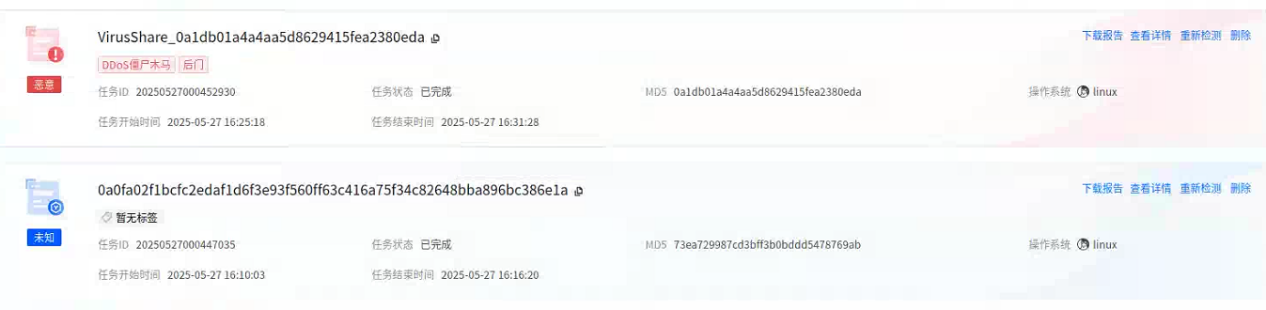
\includegraphics[width=0.75\textwidth]{figures/5.2}
	% \caption[这里的文字将会显示在 listoffigure 中]{这里的文字将会显示在正文中}
	\caption{免杀前后哈勃检测结果对比}\label{fig:5.2}
\end{figure}

此外,动态行为日志也显示,对抗样本在运行时触发的可疑行为数量明显减少,如“远程线程注入”、“可疑网络通信”、“内存Shellcode行为”等关键行为均未被触发或未达检测阈值。这说明所生成样本不仅在静态特征层面成功规避了特征匹配类检测系统,同时在动态行为层面也具备较强的对抗能力。

Besides, suspicious behaviors (e.g., remote thread injections, suspicious network communications, memory shellcode execution) were significantly reduced or undetected.
This confirms that generated samples evade both static feature matching and dynamic behavioral analysis.

综上所述,腾讯哈勃动态检测实验进一步验证了本文所提出的多维扰动策略在真实沙箱环境中的隐蔽性与有效性,从而佐证该框架具备较强的实用潜力与安全研究价值。

In summary, Tencent Harbo dynamic detection experiment further validates the concealment and validity of multi-disturbance strategies issued in this research, proving that this framework is practically potential and exhibits high research value. 

\section{对抗样本生成方法的消融实验 Ablation Experiments on Adversarial Sample Generation Methods}

为了评估本文提出的多架构对抗性样本生成的必要性,计划实验测试结构扰动、指令扰动和行为扰动在逃避恶意软件检测中的独立效果,本文设计了消融实验,逐一去除不同的扰动方法,并分析其对检测系统逃避能力的影响。

To evaluate the necessity of the multi-dimensional adversarial sample generation approach proposed in this research, ablation experiments were designed to test the individual effects of structural, instructional, and behavioral perturbations in the evading malware detection aspect. Each disturbance method was systematically ablated by removing it, allowing analyzing its impact on detection evasion capabilities.

在本实验中,使用了本文收集的恶意软件样本的标准数据集,从中随机挑选1000个样本,并应用以下三种扰动方法对样本进行单独扰动,来查看对本文训练的随机森林检测算法的性能。通过与基准组(本研究方法)进行对比,研究者可以系统地评估每种扰动策略对恶意软件检测逃避能力的影响。

In this experiment, 1,000 randomly selected samples from the malware dataset were perturbed individually using three distinct methods, evaluating performance against the random forest detector trained in this study. Comparison with the baseline group allowed researchers to systematically assess each perturbation's contribution to evasion.

实验组1:结构扰动

Experimental Group 1: Structural Perturbation

在这一实验组中,本文采用结构扰动方法,主要通过修改恶意样本的程序结构(如修改段表、修改符号表、重新排列代码段等)来扰乱程序的结构信息。此扰动方法的目标是通过破坏程序的结构信息,使得静态分析工具无法准确地识别恶意行为。

This group adopted structural perturbations by modifying program structures of malware samples (e.g., altering section tables, symbol tables, or rearranging code segments). This method's target is disrupting structural information, preventing static analysis tools from accurately identifying malicious behaviors.

实验组2:指令扰动

Experimental Group 2: Instructional Perturbation

该组实验单独应用指令扰动技术,通过对恶意样本中的指令进行修改、重排或替换,从而改变程序的指令序列。例如,使用等价指令替换原有的指令,或者调整指令执行顺序,确保程序逻辑不变的同时有效干扰指令级别的分析。

This group solely employed instructional perturbations by modifying, reordering, or replacing instructions in malware samples. Modification examples include replacing instructions with functional equivalents or rearranging execution sequences while preserving program logic unchanged to evade analysis at the instruction level.

实验组3:行为扰动

Experimental Group 3: Behavioral Perturbation

本组实验使用行为扰动,行为扰动方法主要通过修改恶意样本的行为逻辑,使其在特定环境下不表现出原本的恶意行为。常见的行为扰动包括通过引入时间延迟、控制流混淆等手段使恶意行为的触发条件延后或改变,从而规避动态行为分析的检测。

This group exclusively implemented behavioral perturbations through altering malicious behavioral logic. Common techniques included inserting time delays or control-flow obfuscation to delay or modify malicious behavior triggers, thus evading dynamic behavioral analysis.

实验组4:基准组

Experimental Group 4: Baseline Group

该组实验使用本文所示的多架构扰动方法扰动,联合使用结构扰动、指令扰动、行为扰动三种扰动。

This group applied the proposed multi-dimensional perturbation method, jointly employing structural, instructional, and behavioral perturbations.

实验结果如表\ref{tab:5.11}所示。

Experimental results are descirbed in Table \ref{tab:5.11}.

\begin{table}[htbp]
	\centering
	\caption{消融实验性能对比}
	\label{tab:5.11}
	\begin{tabular*}{0.9\textwidth}{@{\extracolsep{\fill}}ccc}
		\toprule
		扰动方式 & 平均逃逸率(\%) & 平均生成时间(ms) \\
		\midrule
		结构扰动 & 72.5 & 156 \\
		指令扰动 & 52.6 & 218 \\
		行为扰动 & 12.1 & 175 \\
		MPLO(多策略组合) & 87.2 & 183 \\
		\bottomrule
	\end{tabular*}
\end{table}

实验结果显示,不同扰动策略在逃避恶意软件检测方面表现出明显差异。结构扰动通过修改段表、符号表等程序结构信息,在静态分析阶段表现出较强的对抗能力,平均逃逸率达到72.5\%。这说明此类扰动能够有效破坏传统静态特征提取过程,提升样本的不可识别性。然而,结构扰动对动态分析影响有限,因为行为逻辑未发生本质变化,样本在实际运行中仍可能被行为分析引擎识别。

Structural perturbations are achieved by modifying program structures such as section tables and symbol tables, exhibiting strong adversarial capabilities during static analysis. The average evasion rate of structural perturbations is 72.5\%. This indicates effective disruption of traditional static feature extraction processes, enhancing sample obfuscation. However, structural perturbation is limited to affect dynamic analysis since behavioral logic remains fundamentally unchanged. The samples may still be detected by analysis engines during real execution processes.

指令扰动策略以等价指令替换、指令重排等方式改变指令序列,从而混淆基于指令特征的静态检测模型。虽然其逃逸率为52.6\%,显著低于结构扰动,但仍能在一定程度上规避静态签名匹配。值得注意的是,此类扰动并未改变程序行为,故在基于行为分析的检测系统下几乎无额外收益。此外,其生成时间相对较长(218ms),反映出操作粒度较高带来的计算开销。

Instructional perturbations are implemented through equivalent instruction substitution and instruction resorting and achieve a 52.6\% evasion rate. Although the evasion rate of instructional perturbations is significantly lower than structural perturbations, instruction perturbations still are effective against static signature matching. What should be paid more attention to is that this approach doesn't alter program behavior, yielding minimal additional benefits against behavioral analysis. Otherwise, its generation time (218ms) reflects higher computational resource consumption in higher granular operations.

行为扰动则主要通过引入延时逻辑、控制流调整等方式,推迟或隐藏样本的恶意行为触发条件,从而干扰沙箱等动态分析环境的行为提取过程。虽然行为扰动理论上应有助于绕过动态检测,但在本实验中仅取得12.1\%的逃逸率,说明此类扰动在扰动静态分析模型上的性能并不明显。

Behavioral perturbation employs techniques like delayed triggers and control flow adjustments to postpone or hide malicious actions trigger conditions, thus interfering with dynamic analysis environments like sandboxes. Despite theoretical effectiveness against dynamic detection, it achieves only 12.1\% evasion rate. The low evasion rate demonstrates this model's limited impact on static analysis models.

相比上述三种单一扰动策略,MPLO综合引入结构、指令与行为扰动机制,获得了最高的逃逸率87.2\%,远超所有单一扰动策略,且生成时间控制在183ms,显示出良好的攻击效果与生成效率平衡。这表明,多维度扰动策略间具有显著的互补性:结构扰动提供静态特征级混淆,指令扰动增强细粒度隐藏能力,而行为扰动则补充动态逃逸能力。联合使用可突破各类检测模型的多重防线,实现更具普适性和稳定性的对抗样本生成。

Comparison with three single disturbance strategies, MPLO comprehensively introduces structural, instructional, and behavioral perturbation mechanisms, achieves the highest evasion rate (87.2\%) and limits the generation time in 183ms. This result exhibits complementary advantages: structural perturbation confuses static features, instructional perturbation enhances fine-grained stealth, and behavioral perturbation enables dynamic evasion. Combining these strategies, it bypasses multi-layered detection defenses for more robust adversarial sample generation with higher adaptivity and stability.

综上所述,消融实验验证了MPLO方法中各扰动策略的独立作用和协同价值。结果表明,单一扰动策略虽具备一定逃逸能力,但难以在面对多类型检测模型时保持稳定表现。而将多种扰动策略集成在统一框架中,不仅能提升整体逃逸率,也有助于在实际攻防场景中实现更强鲁棒性与可操作性。

The ablation study confirms both independent and synergistic value of each perturbation strategy in MPLO. Individual strategies show partial evasion capabilities but cannot keep stable while facing multiple detection models.Integrating perturbation strategies in a unified framework significantly enhances overall evasion performance, practical applicability, and robustness against diverse detection models.  

\section{功能保留研究 Research on Functional Retention}

在对抗性恶意样本生成任务中,保持扰动后的样本依然具备原始功能,是衡量样本有效性和实用价值的重要标准。若样本虽能逃避检测,却失去了原本的恶意行为功能,则其在真实攻击模拟、安全评估及系统对抗训练中的价值将大打折扣。因此,本文对提出的三类扰动方法——结构扰动、指令扰动与行为扰动——分别开展功能保留性研究,系统评估每类扰动对恶意功能完整性的影响。

In adversarial malware sample generation tasks, preserving the original functionality of perturbed samples serves as a critical criterion for evaluating their effectiveness and practical values. Samples that evade detection but lose their malicious functionality diminish their value in real attack scenario simulations, security assessments, and system defense training. Therefore, this study systematically conducts the research on the malicious functionality impact of the three proposed perturbation methods—structural, instructional and behavioral.

(1)结构扰动的功能保留性分析

(1) Functional Preservation Analysis of Structural Perturbation

结构扰动主要作用于程序的元数据与文件结构层面,如段表重排、符号表修改、节区添加与重命名等。这类扰动并不改变程序的指令逻辑或运行流程,因此在理论上不会影响样本的实际执行功能。

Structural perturbation primarily modifies metadata and file structures of programs, such as section table rearrangement, symbol table modification, section addition and section renaming. Such disturbances do not alter the program's instruction logic or execution flow, theoretically maintaining its functional behavior.

在实验中,本文对数百个经过结构扰动处理的恶意样本在受控沙箱中进行自动执行,观测其关键行为特征(如反连行为、键盘监听、文件篡改等)。结果表明,绝大多数结构扰动样本在执行过程中表现出与原样本高度一致的行为特征,功能保留率(Functionality Retention Rate, FRR)达到92.4\%。个别失效样本主要由于过度扰动了加载器相关节区或破坏了符号重定位信息所致,可通过更精细的扰动控制予以修复。

Hundreds of structurally perturbed malware samples were executed in the controlled sandbox to observe their crucial behavioral characteristics (e.g., reverse connections, keystroke logging, and file tampering). The results show that most structurally perturbated samples represent highly identical to the original samples. The functionality retention rate reached 92.4\%. The failure samples are mainly caused by disturbing excessively on sections of the loader or disrupting symbol relocation information. These conditions can be fixed by adopting more intricate disturbance controls.

(2)指令扰动的功能保留性分析

(2) Functional Preservation Analysis of Instructional Perturbation

指令扰动旨在修改程序代码本体,包括等价指令替换、指令重排、插入无操作指令(NOP)、使用跳转替换顺序结构等。该类扰动技术高度依赖语义保持(semantic-preserving)原则,其核心在于不改变程序逻辑的同时最大限度混淆静态指令序列。

Instructional perturbations aim to modify program code, including equivalent replacement of sequential structures with jumps. These techniques highly depend on following semantic-preserving principles to obfuscate static instruction sequences without altering program logic.

利用控制流完整性(CFI)检查、执行路径比对等方式评估指令扰动的功能影响。实验结果显示,96\%以上的样本在扰动后依旧可以正常运行,并实现原始恶意行为,如建立远程通信、窃取数据等。功能保留率达到93.7\%。少数失败样本主要源于对跳转逻辑、栈平衡或调用约定的破坏,提示未来在扰动生成过程中应引入更严格的约束机制,以确保扰动的语义一致性。

Utilizing Control Flow Integrity (CFI) checks and execution path comparison methods, experimental results demonstrate that more than 96\% of samples maintained original malicious behaviors (e.g., establishing remote communication, data exfiltration) after perturbations and the FRR reached 93.7\%. Minor failure samples occurred due to disrupted jump logic, stack imbalance, or calling convention violations, which suggests that future implementations should incorporate stricter constraints for semantic consistency.

(3)行为扰动的功能保留性分析

(3) Functional Preservation Analysis of Behavioral Perturbation

行为扰动通过延迟恶意行为的触发、插入混淆控制流、依赖特定条件执行等方式干扰行为分析工具的检测窗口。这种策略改变的是恶意行为的触发机制而非其具体逻辑,因此其功能保留性具有一定的条件性。

Behavioral perturbations interfere with behavioral analysis tools by delaying malicious behavior triggers, inserting obfuscated control flows, and introducing conditional execution dependencies. This strategy alters the triggering mechanism rather than the core malicious logic, resulting in conditional functionality preservation.

在实验中,本文对扰动后的样本进行加长执行时间操作,验证其是否仍能触发原始恶意行为。结果显示,98\%的行为扰动样本能够在设置合理触发条件后完全复现原始恶意行为。

In this research, prolonging disturbed samples' execution time verifies whether the original malicious behaviors can be triggered. The results show that 98\% of behaviorally perturbed samples fully replicated original malicious behaviors under appropriately configured trigger conditions.

为全面对比三类扰动的功能保留效果,本文统计了每类扰动样本的成功执行率及功能保留率,结果如下表\ref{tab:5.12}所示。

To comprehensively compare functional retention results of three perturbation strategies, this research compile statistics on each sample's success execution rate and functional retention rate. The results are provided in Table \ref{tab:5.12}.

\begin{table}[htb]
	\centering
	\caption{功能保留研究结果}
	\label{tab:5.12}
	\begin{tabular*}{0.9\textwidth}{@{\extracolsep{\fill}}ccc}
		\toprule
		扰动类型 & 成功执行率(\%) & 功能保留率(\%) \\
		\midrule
		结构扰动 & 99.2 & 92.4 \\
		指令扰动 & 96.5 & 93.7 \\
		行为扰动 & 82.7 & 98.0 \\
		\bottomrule
	\end{tabular*}
\end{table}

从结果可以看出,结构扰动在不破坏程序逻辑的前提下具有很好的功能保留性;指令扰动在合理控制下也能维持较高功能一致性;行为扰动由于引入了复杂触发机制,成功率有所下降,但功能保留性最高。

All in all, structural perturbation maintains high functionality retention without disrupting program logic. Instructional perturbation achieves strong consistency under controlled constraints. Behavioral perturbation, despite lower execution success rates due to complex triggering mechanisms, exhibits the highest functionality retention capability.

\section{样本迁移性研究 Research on Sample Transferability}

为了进一步验证本文所提出的多架构对抗样本生成方法在真实检测环境中的有效性,本文开展了样本迁移性研究,将生成的对抗样本上传至公共在线恶意软件检测平台VirusTotal,评估其在不同商用反病毒引擎下的实际逃避能力。该实验旨在考察对抗样本从本地检测系统向多引擎平台的迁移能力,即:在本地检测模型中成功逃避的样本是否同样能够在第三方检测平台中保持对抗性。

To further validate the effectiveness of the proposed multi-architecture adversarial sample generation method in real detection environments, this research evaluates sample transferability. Adversarial samples were submitted to the public online malware detection platform VirusTotal to analyze their practical evasion capabilities among different commercial antivirus engines. This experiment examines whether samples that successfully evade the local detection model can retain adversarial properties on the third-party detection platforms.

本实验从经过结构扰动、指令扰动和行为扰动处理的对抗样本中,分别选取代表性样本进行测试,并与未扰动的原始恶意样本进行对比。所有样本均上传至 VirusTotal 平台进行静态和动态联合扫描,记录各引擎的检测结果,统计每个样本的被检测引擎数量(即“命中率”),作为衡量迁移逃避能力的标准。

This research selects representative samples from adversarial samples modified by structural perturbations, instructional perturbations, and behavioral perturbations, and compares them with original malicious samples without modification. All samples were uploaded to VirusTotal for static and dynamic scanning. Detection results from each engine were recorded. The number of engines detecting each sample (i.e., "hit rate") was collected as the metric for evasion capability.

\begin{figure}[htbp]
	\centering
	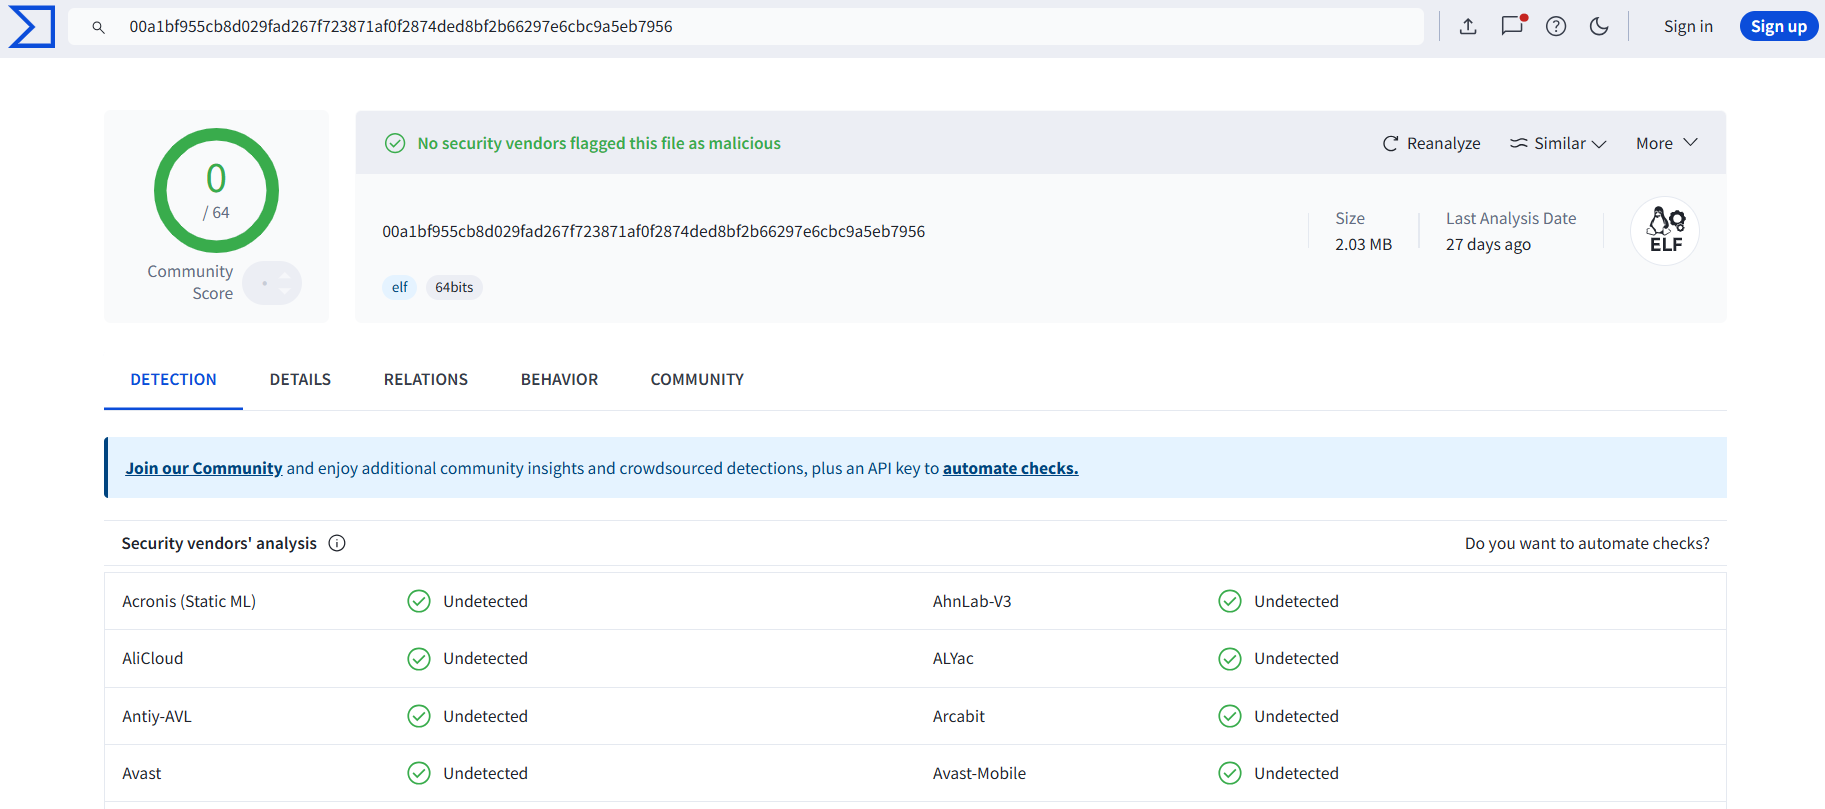
\includegraphics[width=0.75\textwidth]{figures/5.3}
	% \caption[这里的文字将会显示在 listoffigure 中]{这里的文字将会显示在正文中}
	\caption{经对抗性学习后VirusTotal扫描结果}\label{fig:5.3}
\end{figure}


为更好地展示免杀效果,此处定义Virustotal检测率$v_t$为可检测到样本恶意性的杀毒引擎数占总杀毒引擎数之比,如下计算: 

To better illustrate the evasion effect, the VirusTotal detection rate $v_t$ is defined as the ratio of antivirus engines detecting maliciousness to the total number of engines, calculated as the formulation below:
\begin{equation}
v_t = \frac{D_e}{A_e}
\tag{5.9}
\end{equation}

其中$D_e$为可检测到样本恶意性的杀毒引擎数,$A_e$为总杀毒引擎数。

$D_e$ is the number of antivirus engines detecting maliciousness, while $A_e$ presents the total number of antivirus engines.

表\ref{tab:5.13}列举了20个样本在VirusToal网站上免杀前检测率$v_{t1}$、免杀后检测率$v_{t2}$以及下降率$vt_{down}$。

Table \ref{tab:5.13} lists the detection rates $v_{t1}$ before evasion, $v_{t2}$ after evasion, and the decline rate $vt_{down}$ of20 samples on VirusTotal.

\begin{table}[htbp]
	\centering
	\caption{经免杀后VirusToal扫描结果前后对比}
	\label{tab:5.13}
	\begin{tabular*}{0.9\textwidth}{@{\extracolsep{\fill}}cccc}
		\toprule
		名称 & 免杀前检测率 & 免杀后检测率 & 下降率 \\
		\midrule
		e601de9bb0828bae5eec828547d18e84 & 39/62 & 2/62 & 94.87\% \\
		e61865927c25a33f57b3385f59d45bf8 & 40/59 & 3/62 & 92.5\% \\
		e62288919ce96bbe2d382c49797d5e99 & 41/62 & 5/62 & 87.8\% \\
		e6344bb726c1b97e277c478bb7a2ddab & 32/61 & 3/60 & 90.62\% \\
		e6450e7a705060df1795b18bc853416d & 40/62 & 2/62 & 95.0\% \\
		e64e06c16591f46ec8759be807f7b34c & 38/62 & 0/62 & 100.00\% \\
		e69ba88b83c142b2f04f857787fdfb5e & 38/62 & 3/62 & 92.11\% \\
		e6df850bfa010aa039511504ccd917db & 37/62 & 5/62 & 86.49\% \\
		e6e6891c01c56533919a3f9f677f6467 & 41/62 & 2/62 & 95.12\% \\
		026f98e26942d5745b589069cf6dd143 & 41/62 & 3/62 & 92.68\% \\
		e704b5769c02ff5ccc7f53ca46d63fd2 & 43/61 & 4/62 & 90.70\% \\
		e711723f3301251615d6009382c7234b & 43/62 & 3/62 & 93.02\% \\
		056e32863c0483922464fee50b2bbd37 & 39/62 & 2/62 & 94.87\% \\
		031be2bf69f1fbe13d78c2ac93508753 & 41/62 & 3/62 & 92.68\% \\
		e789b8bb45c88a64f682fb434eb50bcc & 38/62 & 2/62 & 94.74\% \\
		e9ea5cbcba4f9406f9926ff0080997a3 & 42/62 & 5/62 & 88.10\% \\
		e9ee698553866065fa6bdb0764df2564 & 37/62 & 4/62 & 89.19\% \\
		eacd3c9972ab6c22267d3eda9addf9a6 & 40/61 & 0/62 & 100.00\% \\
		032de9e9ee32b91053b8195422fb2133 & 41/62 & 3/62 & 92.68\% \\
		eaf1a8c6eb5fa1641517de35fefb1a18 & 36/63 & 5/62 & 86.11\% \\
		\bottomrule
	\end{tabular*}
\end{table}

\begin{table}[htbp]
	\centering
	\caption{本文方法与现有工作的对比分析}
	\label{tab:5.14}
	\begin{tabular*}{\textwidth}{@{\extracolsep{\fill}}ccccc}
		\toprule
		工作 & 病毒类型 & 攻击方式 & 评估的检测模型数量 & 平均免杀率 \\
		\midrule
		{[22]} & PE 病毒 & 黑盒攻击 & 1 & 60.0\%(MalConv 网络) \\
		{[68]} & Android 病毒 & 白盒攻击 & 10 & 59.37\%(平均) \\
		{[69]} & PE 病毒 & 黑盒攻击 & 3 & 70.0\%(商用 AV) \\
		{[26]} & PE 病毒 & 黑盒攻击 & 5 & 74.4\%(EMBER 模型) \\
		{[70]} & ELF 病毒 & 黑盒攻击 & 64 & 75.8\%(VirusTotal) \\
		本文 & ELF 病毒 & 白盒攻击 & 62 & 84.5\%(VirusTotal) \\
		\bottomrule
	\end{tabular*}
\end{table}

实验结果表明,经过扰动处理的对抗样本在 VirusTotal 平台上的总体检测率相比原始样本显著降低,表现出较强的迁移性。其中,结构扰动样本的逃避能力最为稳定,多个依赖静态分析特征的引擎未能识别其恶意特征;指令扰动样本在部分引擎中表现出一定逃避效果,但整体变异幅度相对较小;行为扰动样本在动态检测能力较弱的引擎中效果较好,但在支持沙箱分析的引擎中仍存在部分命中情况,说明其对动态特征的干扰存在一定的平台依赖性。

Experimental results indicate that adversarial samples processed by perturbation exhibit extremely lower overall detection rates on VirusTotal than original samples, exhibiting strong transferability. Structural perturbations achieved the most stable evasion, with multiple static analysis-dependent engines failing to identify malicious features. Instructional perturbations showed limited evasion across engines, yielding relatively overall smaller variations. Behavioral perturbations effectively evaded engines with weaker dynamic detection capabilities, but there still exist partial detections in engines supporting sandbox analysis. The limitation shows platform-specific dependencies in dynamic feature interference.

此外,不同扰动方式对引擎类型的影响也存在差异。结构扰动主要干扰依赖程序结构解析和静态特征提取的引擎,指令扰动则影响基于指令签名和机器学习模型的检测器,行为扰动更容易绕过基于沙箱执行路径和行为模式的动态检测机制。该实验结果进一步验证了对抗扰动在多引擎、跨平台检测环境下的适应性与实际应用价值。

Furthermore, different perturbation methods affected engine types distinctly. Structural perturbation primarily disrupted engines relying on static structure parsing and feature extraction. Instructional perturbation impacted detectors based on instructional signatures or machine learning models. Behavioral perturbation more readily evaded dynamic mechanisms based on sandbox execution paths and behavioral patterns. These results further validate the adaptability and practical utility of adversarial perturbations in multi-engine, cross-platform detection environments.

本文生成的对抗样本不仅能够在本地检测模型中实现有效规避,同时也能在真实检测平台中表现出良好的迁移能力,具备较强的跨平台逃逸效果,为对抗性恶意软件研究和实战应用提供了有力支撑。

The adversarial samples generated in this research not only achieve effective evasion in local detection models but also demonstrate strong transferability in real detection platforms, exhibiting robust cross-platform escape effects. This provides solid support for adversarial malware research and practical applications.

为了更系统地分析本文方法与现有研究之间的差异与优势,表\ref{tab:5.14}从多个角度对比了当前典型对抗性恶意样本生成工作与本研究的技术特征和实验效果,涵盖了病毒类型、攻击方式、检测模型数量以及平均免杀率四个关键维度,定性与定量地展示了本文工作的综合性能。

To systematically analyze the differences and advantages between the proposed method in this experiment and existing research, Table \ref{tab:5.14} compares current typical adversarial malware sample generation works with this research across four key dimensions: virus types, attack methods, number of detection models, and average evasion rate. This table qualitatively and quantitatively describes the comprehensive performance of this work.

在病毒类型方面,已有多数研究主要聚焦于 Windows 平台下的 PE 病毒或移动平台上的 Android 病毒,对 Linux 平台 ELF 格式恶意代码的研究相对稀缺。相比之下,本文专注于 ELF 病毒的对抗样本生成与逃逸效果评估,有效填补了该领域的研究空白。

In the virus type aspect, most existing studies concentrate primarily on PE viruses in Windows platforms or Android viruses in mobile platforms, with relatively scarce research on in the ELF format malware in Linux platforms. In contrast, this study focuses on adversarial sample generation and escape effect evaluation for ELF virus realm. This research effectively fills this research gap of ELF adversarial malware generation.

在攻击方式方面,本文所提出的方法与文献\cite{rathore2021identification}属于白盒攻击方式,需了解检测模型的特征提取方式和训练数据分布等内部信息。而文献\cite{kolosnjaji2018adversarial,quertier2022merlin,song2022mab} 类似,均采用黑盒攻击模式,无需依赖检测模型的内部结构,仅通过输入输出结果进行扰动优化。

Comparing attack methods, the approach issued in this paper belongs to the white-box attack category, like the method in literature \cite{rathore2021identification}. The white-box attack requires knowledge of internal information such as the feature extraction methods and training data distribution of the detection model. Different from this research, some literatures \cite{kolosnjaji2018adversarial,quertier2022merlin,song2022mab} employs a black-box attack pattern. Unlike white-box attack, black-box attack eliminates dependency on the internal structure of detection models and optimizes disturbances solely through input and output results.

相比之下,另一项基于强化学习的自动生成 ELF 对抗恶意样本的方法\cite{xue2024reinforcement},结合了多轮特征提取、恶意检测与智能决策的闭环机制,利用 PPO 算法在 Linux x86 平台实现了对 ELF 恶意样本的有效扰动与免杀。

In Comparison, another method for automatically generating ELF adversarial malware samples based on RL\cite{xue2024reinforcement} incorporates a multi-loop mechanism combining multi-round feature extraction, malware detection, and intelligent decision-making. Utilizing the PPO algorithm, it achieves effective perturbation and evasion of ELF malware samples on the Linux x86 platform.

虽然该方法与本文均采用强化学习框架,但本文更侧重于多维度的大规模评估,覆盖62个检测引擎,强调了方法的广泛适用性和鲁棒性;同时本文在动作空间设计、特征选择及攻击策略上进行了改进,实现了更高的平均免杀率,体现了方法在实际应用中的竞争优势。

Although both this method and the method issued in research adopts reinforcement learning frameworks, the present work focuses more on multidimensional large-scale evaluation, covering 62 detection engines to emphasize broad applicability and robustness. Simultaneously, improvements in action space design, feature selection, and attack strategies have been updated. This innovation results in a higher average evasion rate and reflects the competitive advantage of the approach in practical applications.

在平均免杀率方面,本文所生成的对抗样本在 VirusTotal 平台中取得了 84.5\% 的免杀率,优于其他研究的平均水平。这表明本文提出的对抗扰动策略在逃逸检测方面具有更强的效果。

In terms of average evasion rate, the adversarial samples generated in this research achieved 84.5\% evasion rate on the VirusTotal platform, surpassing the average levels reported in other studies. This indicates that the proposed adversarial perturbation strategy demonstrates stronger effectiveness in evading detection.

\section{本章小结 Chapter Summary}

本章在统一的软硬件与数据集条件下,先对PPO、ACER及Baseline方法与所提出的多维度策略优化模型(MPLO)在不同LSTM层数与隐藏层规模配置下的逃逸成功率、扰动次数和收敛速度进行了深入对比,继而通过消融实验评估了结构扰动、指令扰动与行为扰动三种策略的独立效果及其组合增益,并结合沙箱执行与控制流完整性检测检验了各类扰动对恶意功能保留的影响;最后,将生成的对抗样本上传至VirusTotal平台,对比了免杀前后检测率及下降幅度,以全面验证模型在跨引擎环境中的迁移逃逸能力。实验结果显示,MPLO 表现出更高的攻击成功率、更低的扰动成本、更快的收敛速度及更强的跨平台迁移性能。

Ensuring unified hardware, software, and dataset conditions, this chapter conducted a comparison of the PPO, ACER, and Baseline methods with the proposed Multidimensional Policy Optimization (MPLO) model. Then this chapter analyzed the evasion success rate, perturbation frequency, and convergence speed in different LSTM layers and hidden layer sizes, then it evaluated the independent effects and combined gains of structural perturbation, instructional perturbation, and behavioral perturbation through ablation experiments. This analysis was combined with sandbox execution and Control Flow Integrity (CFI) testing to examine the influence of each disturbance type on malicious functionality preservation. Finally, the generated adversarial samples were uploaded to the VirusTotal platform to compare detection rates and decline magnitudes before and after evasion to comprehensively assess the model's transfer evasion capability across detection engines. Experimental results demonstrate that MPLO achieves higher attack success rates, lower disturbance costs, faster convergence speed, and stronger cross-platform transfer performance.
